% Chapter 23: Changing Magnetic Fields Create Electric Fields
\chapter{Changing Magnetic Fields Create Electric Fields}

\step{A Counterintuitive Opening}

During a nighttime power outage, you may have used an emergency flashlight with no battery inside: shake it vigorously a few dozen times, or turn a handle a few dozen revolutions, and the light comes on for several minutes.

Before jumping to the explanation, appreciate how strange this is. Your knowledge of circuits says that lighting a bulb requires a source of voltage to drive charges around a closed circuit (Chapter 21). A battery maintains a potential difference through chemical processes, but this flashlight has no battery. You have not poured any electricity into it; you merely shook it. All you supplied was effort, mechanical motion. How does mechanical motion become electric current?

The feel of the handle is stranger still. If you have opened one of these flashlights or played with a hand-cranked charger, you will have noticed a distinctly stiff resistance, something invisible working against you. The brighter the connected light, the harder the cranking. Where does that resistance come from? The handle merely turns a magnet near a coil, and magnet and coil never touch.

% BEGIN TRANSLATOR SAFETY NOTE
\textbf{Translator safety note:} Do not test an induction surface with your hand: cookware transfers heat back into the glass, which can remain hot. Observe the appliance's hot-surface indicator and instructions. See \href{https://products.geappliances.com/appliance/gea-support-search-content?contentId=000062465}{GE Appliances surface-temperature guidance}.
% END TRANSLATOR SAFETY NOTE

Related puzzles abound: an induction cooktop's glass surface feels only warm, yet the iron pot on it boils water; a phone on a wireless charging pad receives electricity across a gap, with no connecting wire. Behind them lies one physical law, the true foundation of the electrical age. Without it, there would be no generators, no electrical grid, and no electricity at your wall outlet.

\step{Make a Guess First}

Before continuing, write down your guesses as specifically as possible, so you can check them afterward.

For the flashlight, common guesses include these. First: a tiny battery or wound spring is hidden inside, and shaking is a trick. Second: friction during shaking produces static electricity, like sparks from removing a sweater. Third: the magnet moving through the coil pulls charges out of it. Fourth: the moving magnet somehow pushes charges in the coil.

Try a related question. Find a copper or aluminum tube; neither material is attracted by a magnet, which you can first check with a refrigerator magnet. Drop a small magnet vertically through the tube, then an ordinary iron piece of the same size for comparison. Will the magnet fall as fast, faster, or slower? Most people's intuition says equally fast: copper and aluminum do not attract magnets, and the tube contains only air. What difference could there be?

Finally, a quantitative guess: if you shake twice as fast, does the flashlight produce a little more electricity, twice as much, several times as much, or the same amount?

\step{Hands-on Experiment}

\begin{experiment}[A Magnet's Slow-Motion Fall through a Metal Tube]
\textbf{Materials}: a neodymium magnet (the two strong magnets salvaged from an old computer hard drive work well, or small cylindrical magnets about a centimeter across cost only a few yuan online); aluminum foil rolled into a tube about two centimeters across and fifteen centimeters long, with three or four layers for stiffness; and a similarly sized nonmagnetic object, such as a solid roll of the same foil or a piece of plastic. Caution: neodymium magnets can pinch painfully; keep them away from phones, bank cards, and watches.

\textbf{Procedure}: first bring the magnet to the foil and confirm that there is no attraction. Hold the foil tube vertically and drop the nonmagnetic object in from the top: it falls straight to the bottom with a clack. Now release the neodymium magnet from the same height.

\textbf{What you will see}: the magnet seems transformed, drifting slowly and almost gracefully down, taking several seconds to reach the bottom. A wider tube or a copper tube gives a similar result. Tilt the tube, and the magnet also rolls down slowly.

\textbf{Record your questions}: if magnet and aluminum do not attract, what holds the magnet up? If it is supported and does not accelerate, where has the missing kinetic energy, or gravitational potential energy, gone? Keep these questions: by the chapter's end you should be able to answer them fully.
\end{experiment}

\step{The Old Model Runs into Trouble}

Lay out our existing tools and see whether they suffice. Through Chapter 22, you know three things: charges have electric fields around them, and electric fields exert forces on charges; currents and moving charges have magnetic fields around them; and magnetic fields exert Lorentz forces on moving charges, perpendicular to both their motion and the field, so magnetic fields generally do no direct work on charges.

Check the initial guesses. The first, a hidden battery, can be eliminated experimentally: open the flashlight and find only a magnet, a coil, a few small components, and a small capacitor. The second, frictional static electricity, can also be eliminated. Frictional charging can produce thousands of volts, but only fleeting, hair-thin sparks, never enough to keep a light shining for minutes: static electricity supplies no sustained energy flow. The third, a magnet pulling out charges, makes no sense: magnets attract iron, cobalt, and nickel, not copper, and the flashlight's coil is copper.

That leaves the fourth: the magnet's motion pushes charges in the coil. This heads in the right direction, but ask one level deeper: what is the mechanism? The free charges initially sit quietly among copper atoms, with nearly zero velocity. Yet the Lorentz-force magnitude is proportional to charge velocity: zero velocity means zero magnetic force. How can a magnetic field, powerless over stationary charges, get them moving in an organized current?

Someone may object that the magnet is moving, and its motion carries the charges along. Then consider Faraday's decisive 1831 experiment. He wound coil A around one side of a soft-iron ring and connected it to a battery and switch. On the other side, coil B connected to a galvanometer. The coils did not touch; their only link was the shared iron ring. At switch-on, current appeared in A and a magnetic field appeared in the ring. At that instant B's galvanometer needle flicked. With the switch left closed and the field steady, the needle returned to zero. At switch-off, as the field disappeared, the needle flicked again, oppositely.

Notice particularly that nothing moved throughout the experiment. Coil B was stationary, as were its charges. The only event was that the field passing through it \emph{changed}. The Lorentz force cannot explain this: stationary charges experience no magnetic force. None of our three old tools works. We have found a genuine crack: \textbf{stationary charges beside a changing magnetic field begin moving in an organized direction. Some force we have not yet named must be pushing them.}

\step{Inventing New Concepts}

Faraday had little mathematical training and thought in strongly visual terms. He imagined the space around a magnet filled with magnetic field lines, with patterns of iron filings providing direct evidence of them. Then he proposed a world-changing viewpoint: ignore whether the magnet or coil moves and ask just one question: \textbf{does the total amount of magnetic field passing through a closed loop change?}

That total was later named \textbf{magnetic flux}. Build intuition by imagining the loop as a round fishing net and the field as flowing water. Flux is the amount of water passing through the mesh per unit time: stronger flow and a net facing it more directly let more through. The analogy correctly identifies three factors: field strength, loop area, and how directly the loop faces the field. But its limitation matters: nothing actually flows in a magnetic field. Magnetic flux is not a fluid's flow rate, but an overall account of the spatial field distribution, a purely mathematical bookkeeping device. Nothing flows through your net, yet the account is real.

Faraday concluded that whenever this account changes, whatever causes the change, a driving action on charges appears around the loop. The magnet may approach, the coil may move, the loop may rotate or change area, or the field itself may strengthen or weaken as in the iron-ring experiment. If charges are pushed, an electric field has appeared in the loop. This supplies our new concept: the \textbf{induced electric field}, also called the \textbf{vortex electric field}. A changing magnetic field creates it directly in space, without needing charges as a source.

Its profound differences from the electrostatic fields of Chapters 19 and 20 deserve a list to digest slowly:

\begin{itemize}
\item \textbf{Different sources}: charges produce electrostatic fields; changing magnetic fields produce vortex electric fields, even in space containing no charges.
\item \textbf{Different shapes}: electrostatic field lines begin on positive charges and end on negative ones. Vortex-field lines have no ends, forming closed rings around the region of changing magnetic field, like whirlpools on water.
\item \textbf{Different round-trip accounts}: move a charge around any closed path in an electrostatic field, and the field's total work is exactly zero. That is why we can assign a definite potential to every point (Chapter 20). In a vortex field, the field keeps pushing a charge around the loop, doing total work that is \emph{not zero}. This total round-trip drive is the \textbf{induced electromotive force}.
\end{itemize}

Remember an important consequence of the last point: induced electromotive force is defined \emph{around the whole loop}, not as a potential difference between two points. In a vortex field, asking for the potential at one point has no unique answer. Start there, go around the loop, and return: the field has done net work, so you cannot attach a fixed height label to that point. This is a deep reason behind the book's repeated warning not to confuse electric potential, electric potential energy, and voltage: potential belongs only to electrostatic fields whose lines have beginnings and ends.

For direction, \textbf{Lenz's law} supplies the rule: the effect of an induced current always \emph{opposes} the magnetic-flux change that caused it. As a magnet approaches, the loop pushes it away; as it recedes, the loop tries to retain it. This contrary behavior is not capricious. Energy conservation stands behind it, and we will settle the account mathematically.

\step{The Model in One Sentence}

\begin{oneline}
Changing magnetic flux through a loop produces an induced electromotive force around it. In field language, a changing magnetic field creates circulating electric fields in space. The induced current always opposes the flux change, exactly as energy conservation demands.
\end{oneline}

\step{The Mathematical Translator}

Now translate the intuitions one by one into calculable equations.

\textbf{First: magnetic flux.} Place a flat loop of area \(S\) in a uniform magnetic field of flux density \(B\). Describe how directly the loop faces the field by its orientation: let \(\theta\) be the angle between the field and the loop's normal, the direction perpendicular to its plane. Then the flux is

\[
\Phi = B\,S\cos\theta
\]

in webers (Wb). The left side gives the total magnetic-field account through the loop; the three right-side factors match our intuition: field strength, loop size, and orientation.

\begin{center}
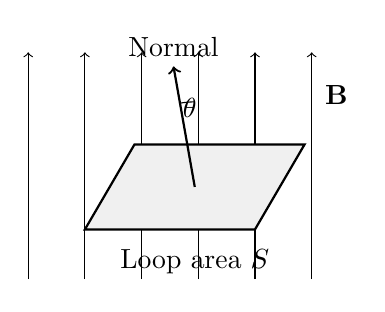
\begin{tikzpicture}[scale=0.9]
  % Uniform magnetic field upward
  \foreach \x in {0,0.8,1.6,2.4,3.2,4.0} {
    \draw[->] (\x,0) -- (\x,3.2);
  }
  \node[right] at (4.05,2.6) {$\mathbf B$};
  % Tilted loop plane
  \draw[thick,fill=gray!12] (0.8,0.7) -- (3.2,0.7) -- (3.9,1.9) -- (1.5,1.9) -- cycle;
  % Normal
  \draw[->,thick] (2.35,1.3) -- (2.05,3.0) node[above] {Normal};
  % Angle between normal and field
  \draw (2.35,2.5) arc[start angle=90,end angle=100,radius=1.2];
  \node at (2.28,2.42) {$\theta$};
  \node[below] at (2.35,0.55) {Loop area $S$};
\end{tikzpicture}
\end{center}

Immediately check special cases. If the loop faces the field directly (\(\theta=0\)), then \(\cos\theta=1\), and flux is maximal at \(BS\): a net facing the current catches most. If the loop lies along the field (\(\theta=90^{\circ}\)), then \(\cos\theta=0\), and flux is zero: a net parallel to the flow catches nothing. Double \(B\) or the area, and flux doubles exactly. All reasonable and consistent with intuition.

\textbf{Second: Faraday's law of electromagnetic induction.} The faster flux changes, the greater the induced electromotive force. A coil with \(N\) turns gives each turn a push, multiplying the effect by \(N\). For the magnitude:

\[
\mathcal{E} = N\,\frac{\Delta\Phi}{\Delta t}
\]

The left side is induced electromotive force, still measured in volts; the right side is flux change per unit time per turn. Notice that the equation contains flux \emph{change} divided by \emph{time}, not flux itself. This is the chapter's easiest point to misremember, and we will return to it shortly.

Check special cases as usual. Hold a magnet still inside the coil: \(\Delta\Phi=0\), so \(\mathcal{E}=0\). However strong the magnet or large the flux, no change means no induction. Insert the magnet with its orientation \emph{reversed}: \(\Delta\Phi\) changes sign, reversing the emf and current, just like the iron-ring experiment's opposite needle flicks at switch-on and switch-off. The shorter the change time \(\Delta t\), the greater the emf: thrusting the same magnet in quickly produces several times the voltage of slow insertion. Direction, zero values, and speed all check out.

\begin{mathbridge}
Using derivatives, Faraday's law becomes more compact:

\[
\mathcal{E} = -N\frac{\mathrm{d}\Phi}{\mathrm{d}t}
\]

The minus sign is no decoration: it is Lenz's law in mathematical form. The induced emf always opposes the flux change. Instead of memorizing a directional mnemonic, ask each time whether the induced current's field replenishes decreasing flux or counters increasing flux.

Another common case gives an immediate result. A straight wire of length \(L\) moves at speed \(v\) perpendicular to a uniform field \(B\), cutting across it. Free charges move with the wire. The Lorentz-force component along the wire pushes positive charge toward one end and negative charge toward the other, until the accumulated charges' electric force balances the magnetic force. The balance \(qE=qvB\) gives the end-to-end voltage:

\[
\mathcal{E} = B\,L\,v
\]

Check: \(v=0\) gives zero, reasonably; reversing \(B\) reverses the emf, reasonably. A longer wire, stronger field, or faster motion gives more voltage, also reasonably. Interestingly, this matches exactly the calculation based on changing loop area and hence changing flux: two ways of accounting for one fact. The coincidence has deeper meaning, to which we return in the model's limits.

For a coil rotating steadily in a uniform field at angular velocity \(\omega\), the flux is \(\Phi=BS\cos\omega t\). Differentiate to obtain

\[
\mathcal{E} = NBS\omega\sin\omega t
\]

The emf varies sinusoidally with time: this is how alternating current is born. The next graph shows it.
\end{mathbridge}

\begin{center}
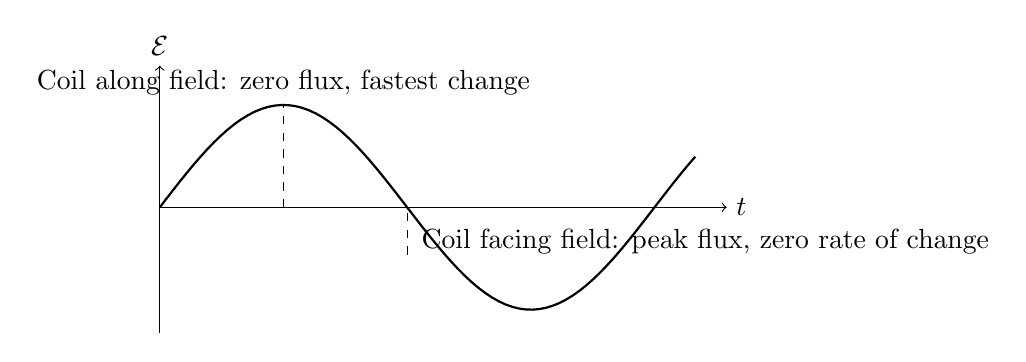
\begin{tikzpicture}[scale=1.0]
  % Axes
  \draw[->] (0,0) -- (7.2,0) node[right] {$t$};
  \draw[->] (0,-1.6) -- (0,1.8) node[above] {$\mathcal{E}$};
  % Sine curve: alternating emf
  \draw[thick,domain=0:6.8,samples=80] plot (\x,{1.3*sin(\x r)});
  % Peak and zero labels
  \draw[dashed] (1.5708,0) -- (1.5708,1.3);
  \node[above] at (1.5708,1.3) {Coil along field: zero flux, fastest change};
  \node[below right] at (3.2,-0.15) {Coil facing field: peak flux, zero rate of change};
  \draw[dashed] (3.1416,-0.6) -- (3.1416,0);
\end{tikzpicture}
\end{center}

Pause to understand this graph: it corrects an extremely common intuitive mistake. The emf crosses zero just when the coil faces the field and flux is \emph{greatest}. But the flux curve is then at its summit, with zero rate of change, so the emf is zero. Conversely, emf peaks when the coil lies along the field and flux is \emph{zero}, because flux then changes fastest. \textbf{Induced emf depends on the rate of flux change, not the flux itself.} However strong the field or large the flux, no change means no induction; however small the flux, rapid change gives strong induction. This explains why a coil translating uniformly through a strong magnetic field carries no current, our counterexample to intuition: intuition expects a strong field to produce electricity; the law requires change.

\textbf{Third: Lenz's law and the energy account.} Translate ``opposes change'' into energy language. Imagine reversing Lenz's law: instead of opposing flux change, the induced current \emph{helps} it. Gently push a magnet toward a closed coil; the induced current pulls it inward, accelerating it, increasing current, strengthening attraction, accelerating it further. You supply nothing, yet the magnet gets faster and the current grows: a perpetual-motion machine with zero input. Energy conservation forbids this, so the induced current must oppose you. Push the magnet inward and its field pushes back; pull it out and the field tries to retain it. The stiff resistance at the flashlight handle is the coil's induced current gripping your magnet through its magnetic field.

The beauty is that the account closes: your work against the resistance equals the energy ultimately dissipated by the current, plus any energy stored. Lenz's law is no new mechanical law, but energy conservation's cashier in electromagnetic induction.

\textbf{Fourth: an estimate with real numbers.} A hand-cranked flashlight typically has a permanent magnet with surface field about \(B\approx 0.3\) tesla, typical of neodymium--iron--boron magnets; coil area about \(S\approx 2\ \mathrm{cm^2}=2\times10^{-4}\ \mathrm{m^2}\); roughly \(N=500\) turns; and gears speeding the magnet to about 20 revolutions per second, giving \(\omega\approx 2\pi\times20\approx 126\) radians per second. The peak emf is

\[
\mathcal{E}_{\max}=NBS\omega \approx 500\times0.3\times2\times10^{-4}\times126\approx 3.8\ \mathrm{V}
\]

A white LED needs about 3 volts, so the scale is just right. Cranking speed enters voltage directly through \(\omega\): turn slowly and the voltage drops below the LED's threshold, dimming the light. This also answers the quantitative initial guess: twice the speed gives roughly twice the voltage, but not simply twice the brightness, since other circuit components also limit current.

\textbf{Fifth: a coil can induce itself---self-induction.} So far flux changes have come from outside. But a coil's own current creates a magnetic field that passes through that same coil. When the current changes, so does its own flux, inducing an emf in the coil that opposes its current change. This is \textbf{self-induction}. Its emf is proportional to the rate of current change, with proportionality constant called the inductance \(L\), measured in henries:

\[
\mathcal{E}_{L} = L\,\frac{\Delta I}{\Delta t}
\]

Inductance behaves much like mechanical inertia: a massive object resists abrupt velocity changes; a highly inductive coil resists abrupt current changes. The analogy works because both store energy, kinetic or magnetic, and both require their state variable to change continuously rather than jump. Starting an object's motion or establishing coil current takes time and work. The difference is that inertial mass stores energy of bodily motion, whereas inductance stores magnetic-field energy; the electrons do not thereby gain mechanical inertia. Once current settles, inductance becomes quiet and stops intervening in the circuit.

Self-induction is no purely academic concept. Old fluorescent lamps use a large inductor called a ballast. At startup, the starter switch opens and forces the inductor current to change abruptly, inducing over a thousand volts that break down the tube's gas and light it. The occasional spark at a household switch opening has the same explanation: rapidly interrupted current makes the wiring's self-inductance generate enough voltage to break down air.

\textbf{Sixth: two coils induce each other---mutual induction and transformers.} Wind two coils on one iron core. A changing current in the first, the primary, changes the core's field; all that changing field passes through the second, the secondary, inducing an emf there. The core confines the field to a closed channel so almost none of the primary flux misses the secondary. An ideal transformer's voltage ratio equals its turns ratio:

\[
\frac{U_1}{U_2}=\frac{N_1}{N_2}
\]

Check special cases: zero secondary turns means zero output, reasonably; a one-to-one turns ratio leaves voltage unchanged, also reasonably. Your phone charger contains a small transformer that first lowers 220-volt mains electricity to a few volts: the primary-to-secondary turns ratio would be about \(44:1\) to obtain 5 volts from 220. The late-night hum of a neighborhood pole-mounted transformer comes from silicon-steel core laminations repeatedly magnetized by a field changing a hundred times per second, expanding and contracting slightly. You are effectively hearing the changing magnetic field itself.

\textbf{Seventh: direct current, alternating current, and the next circuit bridge.} Batteries supply direct current: voltage keeps its direction and charges flow steadily one way. A rotating coil produces electricity whose direction repeatedly reverses. China's mains supply completes 50 cycles per second, with current reversing 100 times per second: alternating current. Why does the grid use AC? The core reason belongs to this chapter: \emph{transformers work only with changing magnetic fields}. DC produces a constant field; apply it to a transformer primary and the secondary receives nothing except at connection and disconnection. Only AC can be conveniently stepped up or down with transformers. Power stations raise voltage to hundreds of thousands of volts for long-distance transmission, reducing current and wire heating, then lower it near your neighborhood. Induction makes not only generation, but practical and economical transmission possible.

Pause to see what power stations actually do. Except for photovoltaic panels, almost every human method of generating electricity, whether hydroelectric, fossil-fueled, nuclear, or wind, ends with the same operation: continuous relative rotation of magnets and coils. Rivers turn water turbines, high-pressure steam turns steam turbines, and wind turns wind turbines. Fossil-fuel plants burn coal and nuclear plants burn uranium; the resulting heat first boils water, whose steam then drives turbines. The route sounds comically indirect, but each step has a reason. Coal and uranium supply heat, which cannot directly become electric current, while a rotating coil plus magnetic field is currently our most economical large-scale conversion interface. A million-kilowatt power station is essentially an enormous version of this chapter's demonstration, driven by rivers or steam.

Inductance completes the circuit's three basic players: resistance resembles friction, irreversibly dissipating electrical energy as heat; capacitance resembles a spring (Chapter 21), storing charge and electric-field energy; inductance resembles an inertial flywheel, storing magnetic-field energy. Their combinations lead to later bridges in the book. Resistance plus capacitance (RC) determines charging and discharging rates, explaining why a camera flash needs time to recharge. Resistance plus inductance (RL) determines how quickly current starts and stops. Inductance, capacitance, and a little resistance (RLC) reproduce spring, inertia, and damping electrically: current oscillates between capacitor and inductor as electric- and magnetic-field energies exchange, like a swing alternating kinetic and potential energy. Tuning a radio selects the resonance of just such an oscillation. We will return to this thread with Maxwell's equations and electromagnetic waves in Chapters 24 and 25.

\step{The Model's Limits}

Every important formula must answer when it holds and when it fails. Induction particularly deserves care, because its validity is surprisingly broad and its common misuses surprisingly numerous.

\textbf{Scope.} Experimentally, Faraday's law applies generally to macroscopic loops. Flux change may arise from changes in field strength, loop area, orientation, movement through a field, or any combination. The law applies regardless of material, temperature, or whether a load is connected. It works in geomagnetic recording coils at underground observatories and precision induction probes in particle accelerators. There is no field-strength ceiling beyond which it fails: hospital MRI fields of several teslas and the unimaginable fields around pulsars obey the same law.

\textbf{Misuse one: assuming a field means induction.} We have stressed this already, but it merits another warning sign: a stationary or uniformly translating coil in a steady strong magnetic field has no induced current. The only question is whether flux through the loop changes, not whether the field is strong. Perhaps the mistaken intuition confuses strength with activity: a stationary mountain is majestic, but pushes nothing.

\textbf{Misuse two: saying Lenz's law opposes a magnet's motion.} More precisely, it opposes flux \emph{change}. A magnet entering a coil is repelled and one leaving is attracted, but a magnet stationary at the exact center feels no force. Lenz's law watches change, not motion; motion merely happens to imply change in most cases.

\textbf{Misuse three: assuming the flux rule solves every circuit problem.} A famous counterexample is Faraday's disk, also humanity's first generator. A copper disk rotates in a magnetic field, with brushes at the axle and rim carrying current outward. The disk's location stays fixed, and the flux through the whole apparatus seems unchanged, yet current really flows. The difficulty lies in selecting the loop: part of the current path lies inside the rotating disk and cuts across the field with it. Here a motional-emf calculation, based on a conductor cutting field lines, is clearer; blindly applying loop-flux change creates contradictions. The law is not wrong. Rather, ``loop'' needs careful definition when moving conductor boundaries are involved.

\textbf{Deeper down: the two kinds of induction are one phenomenon.} Flux can change because a coil moves through a magnetic field, giving motional induction explained by the Lorentz force, or because the field itself changes, requiring a vortex electric field. But who moves depends on the reference frame. Bring a magnet toward a stationary coil or a coil toward a stationary magnet, and the coil experiences the same effect. Einstein opened his 1905 relativity paper with this magnet--conductor asymmetry: the old theory offered two explanations of the same event. Demanding one account of nature led him to special relativity, in which electric and magnetic fields transform into one another between frames. We continue that story in Chapter 38.

\textbf{The chapter's biggest hint of what follows.} We have said that changing magnetic fields create electric fields. Maxwell stared at that statement and asked a question of symmetry: what about changing electric fields? He boldly added the other half: changing electric fields create magnetic fields too. This addition directly predicted electromagnetic waves and ultimately revealed that light is an electromagnetic wave. That is the story of Chapters 24 and 25.

\begin{challenge}
In field language, the vortex electric field has this property: around any closed loop, the electric field's accumulated component along the path, its circulation, equals minus the rate of change of magnetic flux through the loop:

\[
\oint\mathbf{E}\cdot\mathrm{d}\mathbf{l}=-\frac{\mathrm{d}\Phi_B}{\mathrm{d}t}
\]

Electrostatic circulation is identically zero, making the electrostatic field conservative and allowing a potential. Vortex-field circulation is nonzero, so that field is not conservative and electric potential fails for it. This contrast is the full content of Faraday's equation in Maxwell's equations and the key to the displacement-current addition in Chapter 24. Another interesting question: if vortex-field lines form closed rings, does a changing magnetic field in vacuum, far from every wire, really have an electric field around it? Experiments say yes. A betatron uses a changing field in a ring-shaped vacuum chamber to accelerate electrons almost to light speed, with no wire touching them.
\end{challenge}

\step{Explaining the Opening Phenomenon}

Return with the full model to the opening phenomena and settle their accounts one by one.

\textbf{The hand-cranked flashlight.} You turn the handle, and gears spin a permanent magnet rapidly beside a coil. Flux through the coil repeatedly grows, shrinks, and reverses dozens of times per second, inducing an emf that repeatedly reverses: a little alternating current. Diodes allow current in only one direction, straightening the AC and charging a small capacitor. That is why the light remains on for minutes after you stop: stored capacitor charge keeps supplying it. The resistance in your hand is Lenz's law visiting personally. Once current flows, its magnetic field exerts an opposing torque on the rotating magnet. Your work against it follows the chain mechanical energy--electrical energy--light and heat, becoming the lamp's light without a penny missing. A brighter connected lamp needs more current, producing more opposing torque and harder cranking. Energy conservation does not bargain.

\textbf{The magnet falling through aluminum.} As it falls, the flux through each little ring of tube wall changes: decreasing above the magnet and increasing below. Aluminum conducts well, so this changing flux induces circulating wall currents, aptly called \textbf{eddy currents}, like whirlpools in water. By Lenz's law, their field always opposes the magnet's motion, pulling from above and pushing from below. The net upward force makes the magnet drift down slowly. Its lost gravitational potential energy becomes Joule heat in the aluminum's resistance. The tube warms slightly, though usually too little to notice. Copper and aluminum do not attract a magnet, yet can brake it: their bridge is induction, not magnetism. The initial guess of equal falling speeds failed by confusing no magnetic attraction with no interaction.

% BEGIN TRANSLATOR SAFETY NOTE
\textbf{Translator safety note:} The source's ``not very hot'' conclusion is not a safety guarantee. Heat from cookware can leave the glass hot after cooking; do not touch it until it has cooled. See \href{https://products.geappliances.com/appliance/gea-support-search-content?contentId=000062465}{GE Appliances hot-surface guidance}.
% END TRANSLATOR SAFETY NOTE

\textbf{The induction cooktop.} Beneath the glass is a flat copper coil carrying high-frequency AC that changes more than twenty thousand times per second. An iron pot above it develops strong eddy currents in its metal base. Resistance makes these currents generate heat directly inside the pot bottom. Heat originates in the pot; the nearly nonconducting glass develops no eddy currents of its own and is merely warmed by the pot. That is why the water can boil while the surface remains not very hot. Pure copper and aluminum pots have resistivities too low for efficient heating despite large eddy currents, so most induction cooktops detect them and refuse to operate. Reverse the same idea and you get a metal detector: a security gate's coil emits a changing field, inducing eddy currents in your keys; the instrument detects their returning magnetic field. What the gate hears is the answer from induced currents on your person.

\textbf{Wireless charging and electric guitars.} We also began with a phone charging across a gap. Now you can see through it. The pad contains a high-frequency AC coil, and another coil sits behind the phone's back. Separated by a few millimeters of air, they form a transformer without an iron core: mutual induction. Without a core to confine the field, much flux leaks away, so efficient charging requires close contact and alignment; move the phone away and efficiency plummets. Transformer physics plays out again in your palm. Another instrument deserves a look: an electric guitar's pickup is a small magnet wrapped in thousands of turns of fine wire beneath the strings. Ferromagnetic strings vibrate and change the nearby field distribution, varying the coil's flux and producing an electrical signal synchronized with the vibration. String motion first becomes flux change, then current variation, and finally sound through an amplifier. Our old friend the guitar, already encountered with tension and standing waves, reveals another layer in electromagnetism.

\step{Thought Experiments and Challenges}

\begin{thought}[An Electricity-Generating Tether in Space]
Push induction to an extreme scale: what happens if a twenty-kilometer wire hangs from a spacecraft orbiting Earth? Moving with the spacecraft at about 7.7 kilometers per second, it sweeps across Earth's field of about \(3\times10^{-5}\) tesla. The motional-emf estimate is

\[
\mathcal{E}=BLv\approx 3\times10^{-5}\times2\times10^{4}\times7.7\times10^{3}\approx 4.6\times10^{3}\ \mathrm{V}
\]

Thousands of volts, enough to break down air! This is no mere fantasy. In 1996, a US space shuttle conducted a tethered-satellite experiment, towing a satellite on a roughly twenty-kilometer tether to generate electricity in space. With most of the tether deployed, the experiment measured voltages of several thousand volts. Unfortunately, the tether then broke accidentally and the satellite drifted away. Think: even if it had remained intact, where would current come from and where would it go? The wire's ends were not directly connected into a loop. The circuit had to close through thin plasma in Earth's upper atmosphere: one tether end collected electrons from the plasma, and the other emitted them back into space with an electron gun. Even in orbit four hundred kilometers up, current must form a loop.
\end{thought}

\begin{puzzles}
\item A closed coil with \(N\) turns and resistance \(R\) experiences a flux change from \(\Phi_1\) to \(\Phi_2\). In one trial the change takes one second; in another, one hundredth of a second. Which sends more \emph{total charge} through a given cross section? (Hint: current is \(I=\mathcal{E}/R\), and total charge is current accumulated over time. Substitute \(\mathcal{E}=N\Delta\Phi/\Delta t\) and see whether \(\Delta t\) cancels. Pulling quickly gives more current for less time; pulling slowly gives less current for longer. Add up the account.)
\item Two identical aluminum tubes stand vertically, but one has a narrow vertical slit running its full length. Drop identical magnets into them simultaneously. Which reaches the ground first? (Hint: eddy currents need \emph{closed} circles around the wall. What does a slit do to those circles? Take one more step: if the magnet in the slit tube nearly free-falls, at which level did your initial intuition fail?)
\item Why are transformer cores built from many thin silicon-steel sheets coated with insulating varnish, instead of one solid iron block? (Hint: the core's field changes a hundred times per second, and iron itself conducts. Looking along the field, how large an eddy-current loop could a solid block contain? What happens to the loops when you divide it into insulated sheets? This is the same idea as the slit in Challenge 2.)
\item Suppose Earth's field, about \(5\times10^{-5}\) tesla, reverses completely in one minute. What voltage appears across a discarded 100-turn coil of area 1 square meter on your desk? Could it electrocute someone? (Hint: reversal changes flux from \(+BS\) to \(-BS\), so \(\Delta\Phi\) is \(2BS\). Calculate the scale before concluding: induction is everywhere, but whether an effect exists and how large it is are separate questions.)
\end{puzzles}
